% This must be in the first 5 lines to tell arXiv to use pdfLaTeX, which is strongly recommended.
\pdfoutput=1
% In particular, the hyperref package requires pdfLaTeX in order to break URLs across lines.

\documentclass[11pt]{article}

% Remove the "review" option to generate the final version.
\usepackage[review]{ACL2023}

% Standard package includes
\usepackage{times}
\usepackage{latexsym}

% For proper rendering and hyphenation of words containing Latin characters (including in bib files)
\usepackage[T1]{fontenc}
% For Vietnamese characters
% \usepackage[T5]{fontenc}
% See https://www.latex-project.org/help/documentation/encguide.pdf for other character sets

% This assumes your files are encoded as UTF8
\usepackage[utf8]{inputenc}

% This is not strictly necessary, and may be commented out.
% However, it will improve the layout of the manuscript,
% and will typically save some space.
\usepackage{microtype}

% This is also not strictly necessary, and may be commented out.
% However, it will improve the aesthetics of text in
% the typewriter font.
\usepackage{inconsolata}

%% Use the graphicx package to include figures.

\usepackage{graphicx}


% If the title and author information does not fit in the area allocated, uncomment the following
%
%\setlength\titlebox{<dim>}
%
% and set <dim> to something 5cm or larger.

\title{A Case Study Replicating Calibration of Large Language Models on Open Models and Datasets}

% Author information can be set in various styles:
% For several authors from the same institution:
% \author{Author 1 \and ... \and Author n \\
%         Address line \\ ... \\ Address line}
% if the names do not fit well on one line use
%         Author 1 \\ {\bf Author 2} \\ ... \\ {\bf Author n} \\
% For authors from different institutions:
% \author{Author 1 \\ Address line \\  ... \\ Address line
%         \And  ... \And
%         Author n \\ Address line \\ ... \\ Address line}
% To start a seperate ``row'' of authors use \AND, as in
% \author{Author 1 \\ Address line \\  ... \\ Address line
%         \AND
%         Author 2 \\ Address line \\ ... \\ Address line \And
%         Author 3 \\ Address line \\ ... \\ Address line}

\author{Aakarsh Nair\\
  University of Tuebingen / Geschwister-Scholl-Platz, 72074 Tübingen\\
  \texttt{aakarsh.nair@aakarsh.nair@student.uni-tuebingen.de} 
  Second Author \\
  Affiliation / Address line 1 \\
  Affiliation / Address line 2 \\
  Affiliation / Address line 3 \\
  \texttt{email@domain} \\}

\begin{document}
\maketitle

\begin{abstract}
The popularity of large language models has lead to a growing 
need to characterize their behavior and understanding 
beyond the generation grammatical sentences. In this study we 
attempt to replicate and extend the calibration study of 
\cite{kadavath2022language} on open models and datasets, 
attempting compare model reported response probabilities to 
their actual calibration, that is the certainty with which a model answers 
a question with a given completion and the probability that the 
model is answering the question correctly. 
\end{abstract}

\section{Introduction}

%% Introduction, motivation and explanation of the research question in the context 
%% of the field / the class, explaining why it is intersting / novel in comparison 
%% to extant related work. Note that it is NOT mandatory to include an 
%% exhaustive literature review; it is sufficient to mention relevant work 
%% from the project proposals and the class materials

\section{Method}

\subsection{Introduction}

We measure the calibration in keeping with the methodology presented 
in  \cite{kadavath2022language}. The model is queried in either a
0-shot or 5-shot manner. The transformer model is given a question 
prompt  with the each of the multiple choice options.  In the 5-shot 
methodology, in addition to the question under test we proceed the 
question with 4 additional questions with in the same multiple 
choice format in order to provide the model with enough context to 
understand the expected format for answering the question.

For each prompt completion pair we compute the log probability of 
the completion normalized by its completion length. 


The computed probabilities are then grouped in bins in $10$ bins from 
$0$ to $1$ were we compute the average frequency of answering 
correctly for each bin. 

For ideal calibration, that is when the model completion probability aligns
closely with the actual probability of answering the question correctly, these 
two computed probabilities must be equal, thus a ideal calibration would be 
represented  by a line of slope $1$ in the calibration plot. Negative 
and positive deviations thus represent a model which is under-confident 
or over-confident  in its answers respectively.

\subsection{Dataset}

The Measuring Massive Multitask Language Understanding (MMLU) 
\cite{hendrycks2021measuring} is a massive dataset of multiple choice 
questions which covers 57 tasks in various subjects including 
elementary mathematics, US history, computer science, law, and more. It 
serves as a challenging dataset for most modern large language models and can be used to evaluate their calibration.

\subsection{Model Calibration By Number of Parameters}

We compare the calibration of the Llama \cite{touvron2023llama} model 
7b-chat and 13b chat models for answering multiple choice questions in 
figure ... 

We note that that the calibration of the model while not perfect improves 
with the size of the model with the 13b-chat model being better calibrated 
and closer to the ideal calibration line than the 7b-chat model. Thus we 
note that models sizes improves not only the performance of the model but
the calibration of the model as well.

\begin{figure}
  \centering
  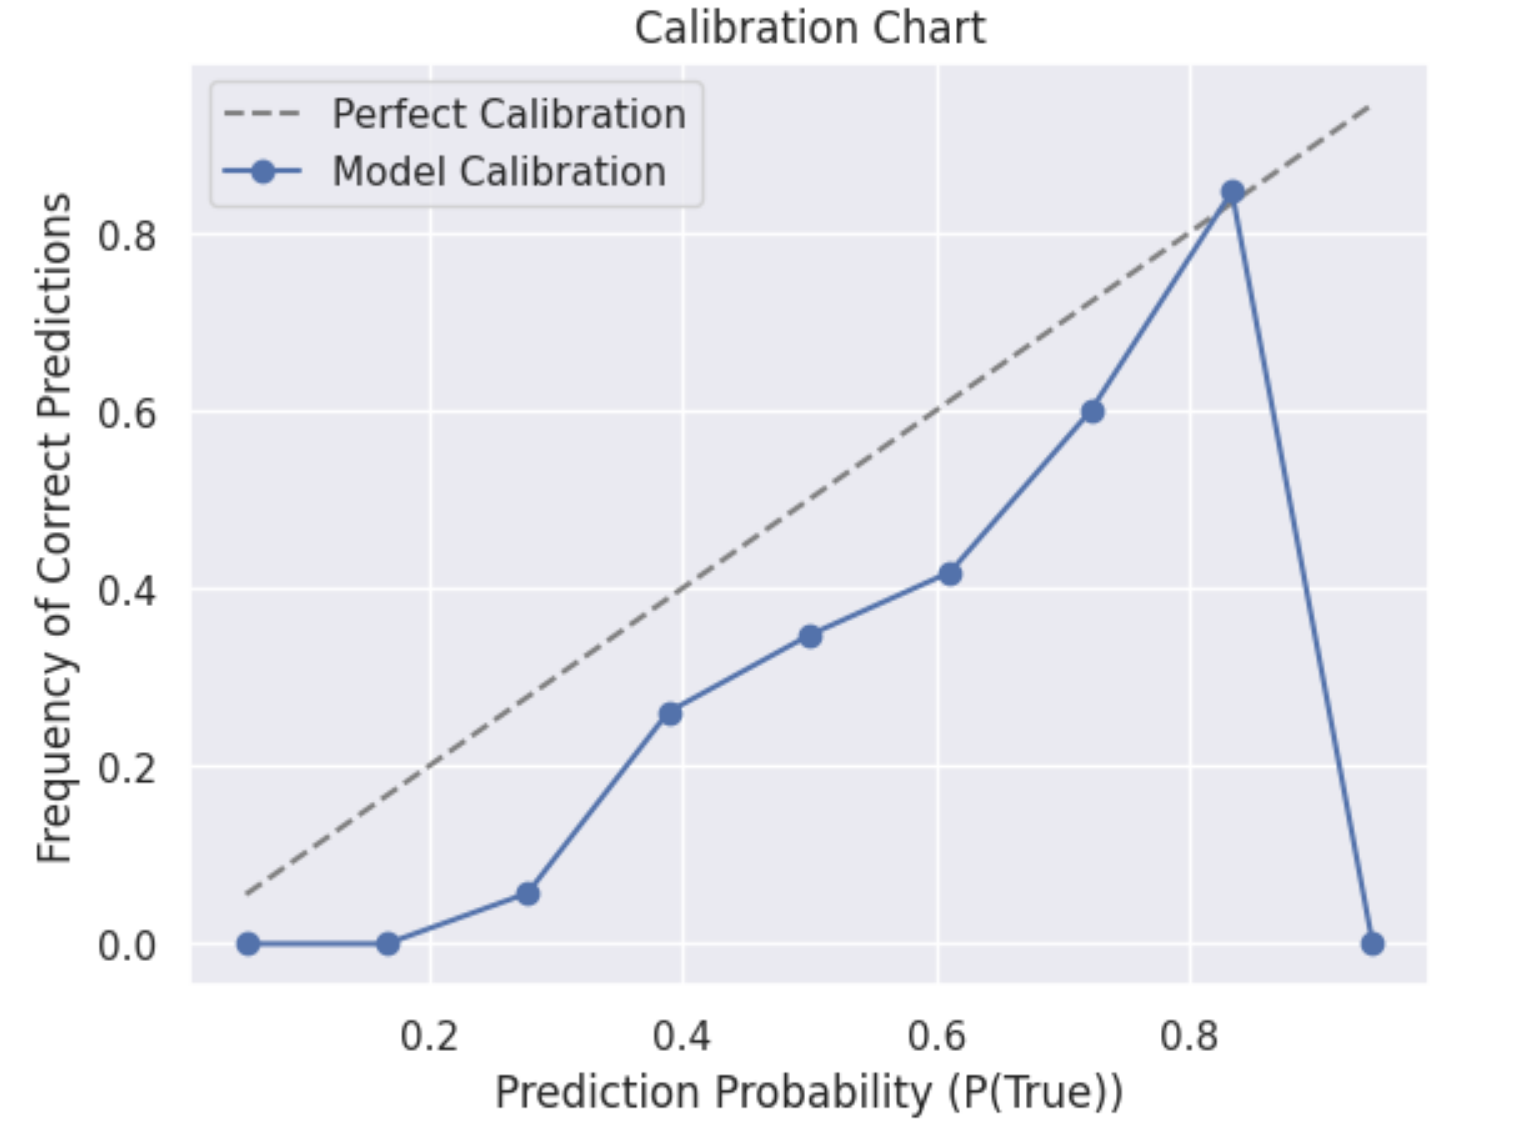
\includegraphics[width=0.5\textwidth]{figures/mmlu-13b-chat.png}
  \caption{Calibration of the 13b-chat model on the MMLU dataset, we 
  note that it is closer, in calibration than the 7b-chat model. }
\end{figure}

\subsection{Model Calibration By Number By Fine Tuning}  

\subsection{Model Calibration By Number By Subject Specialization}  

\section{Results}
\begin{table*}
\centering
\begin{tabular}{lll}
\hline
\textbf{Output} & \textbf{natbib command} & \textbf{Old ACL-style command}\\
\hline
\citep{ct1965} & \verb|\citep| & \verb|\cite| \\
\citealp{ct1965} & \verb|\citealp| & no equivalent \\
\citet{ct1965} & \verb|\citet| & \verb|\newcite| \\
\citeyearpar{ct1965} & \verb|\citeyearpar| & \verb|\shortcite| \\
\citeposs{ct1965} & \verb|\citeposs| & no equivalent \\
\citep[FFT;][]{ct1965} &  \verb|\citep[FFT;][]| & no equivalent\\
\hline
\end{tabular}
\caption{\label{citation-guide}
Citation commands supported by the style file.
The style is based on the natbib package and supports all natbib citation commands.
It also supports commands defined in previous ACL style files for compatibility.
}
\end{table*}
The first line of the file must be
\begin{quote}
\begin{verbatim}
\documentclass[11pt]{article}
\end{verbatim}
\end{quote}
To load the style file in the review version:
\begin{quote}
\begin{verbatim}
\usepackage[review]{ACL2023}
\end{verbatim}
\end{quote}
For the final version, omit the \verb|review| option:
\begin{quote}
\begin{verbatim}
\usepackage{ACL2023}
\end{verbatim}
\end{quote}
To use Times Roman, put the following in the preamble:
\begin{quote}
\begin{verbatim}
\usepackage{times}
\end{verbatim}
\end{quote}
(Alternatives like txfonts or newtx are also acceptable.)
Please see the \LaTeX{} source of this document for comments on other packages that may be useful.
Set the title and author using \verb|\title| and \verb|\author|. Within the author list, format multiple authors using \verb|\and| and \verb|\And| and \verb|\AND|; please see the \LaTeX{} source for examples.
By default, the box containing the title and author names is set to the minimum of 5 cm. If you need more space, include the following in the preamble:
\begin{quote}
\begin{verbatim}
\setlength\titlebox{<dim>}
\end{verbatim}
\end{quote}
where \verb|<dim>| is replaced with a length. Do not set this length smaller than 5 cm.

\section{Discussion}

\section{Conclusion}
\label{sec:bibtex}

\section{Acknowledgements}

\section{References}

\section{Acknowledgements}

% Entries for the entire Anthology, followed by custom entries
\bibliography{anthology,custom}
\bibliographystyle{acl_natbib}

\appendix

\section{Appendix}
\label{sec:appendix}

This is a section in the appendix.

\end{document}
